\section{Examples (for the System Model section}

\begin{example}
\label{ex:first}
Consider a manufacturing system consisting of three cells $V=\{v_1, v_2, v_3\}$.
The plant can be represented as a graph $G=(V,E)$ shown as follows: %in Figure~\ref{fig:ex_plant_graph}.

\begin{figure}[h]
%\vspace{-\baselineskip}
\centering
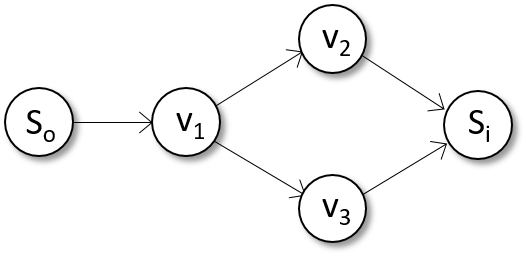
\includegraphics[width=0.5\columnwidth]{Figures/ex_plant_graph}
%\vspace{-\baselineskip}
%\caption{TBD (The figure will be converted to PDF later when it is final.}
\label{fig:ex_plant_graph}
%\vspace{-1\baselineskip}
\end{figure}

\noindent
Note that $S_o$ is the source where widgets enter the plant and $S_i$ is the sink where widgets finish the required operations and leave the plant. The supported operations for each cell are given in the following table:

\begin{table}[h]
\centering
%\caption{My caption}
\begin{tabular}{|l|l|}
\hline
Cell & Supported Operations \\ \hline \hline
$v_1$ & $op_1$         \\ \hline
$v_2$ & $op_2$         \\ \hline
$v_3$ & $op_2, op_3$         \\ \hline
\end{tabular}
\end{table}

That is, $OP=\{op_1, op_2, op_3\}$, $L_{v_1}=\{op_1\}$, $L_{v_2}=\{op_2\}$ and $L_{v_3}=\{op_2, op_3\}$. 
\hl{CY: The operation time will be given if it is needed in this example.}

From the plant introduced in Example~\ref{ex:simple_plant}, let's further consider two types of widgets, $W=\{w_1, w_2\}$, being fabricated in this plant.
Their requirements are given as graphs as follows:

\begin{figure}[h]
%\vspace{-\baselineskip}
\centering
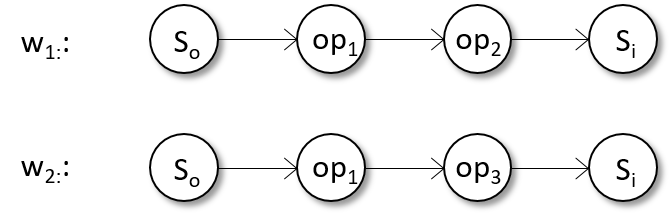
\includegraphics[width=0.65\columnwidth]{Figures/ex_widget_requirements}
%\vspace{-\baselineskip}
%\caption{TBD (The figure will be converted to PDF later when it is final.}
\label{fig:ex_widget_requirements}
%\vspace{-1\baselineskip}
\end{figure}


\end{example}